\documentclass[14pt]{article}

\usepackage[utf8x]{inputenc}
\usepackage[russian]{babel}
\usepackage{graphicx}
\graphicspath{{images/}}
\DeclareGraphicsExtensions{.pdf,.png,.jpg}

\usepackage{amsmath}
\usepackage{pgfplots}

\usepackage{geometry} % Меняем поля страницы
\geometry{left=2cm}% левое поле
\geometry{right=1.5cm}% правое поле
\geometry{top=2cm}% верхнее поле
\geometry{bottom=2cm}% нижнее поле

\renewcommand{\theenumi}{\arabic{enumi}}
\renewcommand{\labelenumi}{\arabic{enumi}}
\renewcommand{\theenumii}{.\arabic{enumii}}
\renewcommand{\labelenumii}{\arabic{enumi}.\arabic{enumii}.}
\renewcommand{\theenumiii}{.\arabic{enumiii}}
\renewcommand{\labelenumiii}{\arabic{enumi}.\arabic{enumii}.\arabic{enumiii}.}

\begin{document}
\begin{titlepage}
	\begin{center}
		\fontsize{18pt}{20pt}\selectfont
		\textbf{Работа 4.7.1.}	
	
		\vspace{5cm}
		\fontsize{24pt}{25pt}\selectfont
		Двойное лучепреломление
	\end{center}
	\begin{flushright}
		\fontsize{18pt}{20pt}\selectfont
		\vspace{14cm}
		\hspace{-3cm}
		\textit{Корнеев Е.С.}
	\end{flushright}		
\end{titlepage}

\begin{center}
	\fontsize{16pt}{18pt}\selectfont
	Двойное лучепреломление
\end{center}


\fontsize{14pt}{16pt}\selectfont

\vspace{0.5cm}
\textbf{Цель работы:} изучение зависимости показателя преломления
необыкновенной волны от направления в двоякопреломляющем кристалле;
определение главных показателей преломления no — обыкновенной
и ne — необыкновенной волны в кристалле1; наблюдение эффекта
полного внутреннего отражения.

\vspace{0.5cm}
\textbf{В работе используются:} гелий-неоновый лазер, вращающийся столик
с неподвижным лимбом, призма из исландского шпата, поляроид.

\vspace{1cm}

При падении световой волны на границу изотропной среды в этой
среде от границы распространяется одна волна. Если среда анизотропна,
то в ней в общем случае возникают две волны, распространяющиеся
от границы в разных направлениях и с разными скоростями. Это явление
называется \textsl{двойным лучепреломлением}. Оно было открыто Бартолинусом
в 1669 г. в кристаллах исландского шпата, призма из которого
исследуется в нашей работе.

\textbf{Плоские волны в кристаллах.} Фундаментальные уравнения Максвелла
справедливы без всяких изменений и в кристаллических средах.
В отсутствие электрических зарядов и токов они имеют вид
\begin{equation}
rot\vec{H} = \frac{1}{c}\frac{\partial\vec{D}}{\partial t},~~~~~rot\vec{E} = -\frac{1}{c}\frac{\partial\vec{B}}{\partial t}
\end{equation}

Если среды прозрачны и однородны, то в них могут распространяться
плоские монохроматические волны. Запишем такую волну в комплексном
виде:
$$
	\vec{E} = \vec{E_0}e^{i(\omega t - \vec{k}\vec{r})};~~\vec{B} = \vec{H} = \vec{H_0}e^{i(\omega t - \vec{k}\vec{r})};~~\vec{D} = \vec{D_0}e^{i(\omega t - \vec{k}\vec{r})}
$$

Здесь $\omega$ — круговая частота, $\vec{k}$ — волновой вектор, а амплитуды $E_0, D_0, H_0$ постоянны. Вектор $\vec{B}$
совпадает с $\vec{H}$, так как $\mu$ = 1. Дифференцируя
по времени, получаем $\partial\vec{D}/\partial t = i\omega\vec{D}$, т.е. операция дифференцирования
сводится в этом случае к умножению на $i\omega$. Аналогично дифференцирование
по координатам $x, y, z$ сводится к умножению на $−ikx, −iky, −ikz$.
Заметив это, получаем
$$
	rot\vec{H} = -i[\vec{k}\vec{H}]
$$

и аналогично для $rot\vec{E}$. В результате (1) перейдут в
$$
	[\vec{k}\vec{H}] = -\frac{\omega}{c}\vec{D},~~[\vec{k}\vec{E}] = -\frac{\omega}{c}\vec{B}
$$

Введем единичный вектор нормали
$\vec{N}$ к фронту волны и скорость распространения фронта в направлении этой нормали $v$. Тогда $\vec{k} = \frac{\omega}{v}\vec{N}$
предыдущие соотношения перейдут в
\begin{equation}
	\vec{D} = -\frac{c}{v}[\vec{N}\vec{H}];~~\vec{B} = \frac{c}{v}[\vec{N}\vec{E}]
\end{equation}

Отсюда видно, что векторы
$\vec{D}, \vec{H}, \vec{N}$ взаимно перпендикулярны. Значит,
плоские волны в кристалле поперечны в отношении векторов $\vec{D}$ и $\vec{H}$.
Однако в общем случае они не поперечны в отношении вектора $\vec{E}$.

\begin{figure}[h!]
	\center{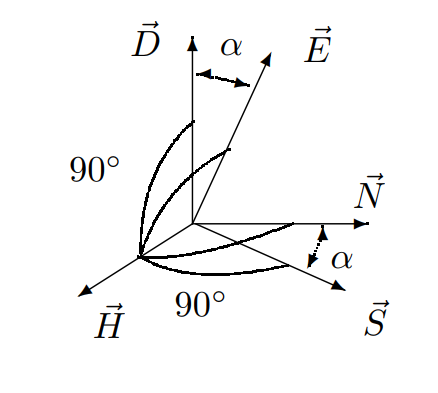
\includegraphics[width = 8cm]{1}}
	\caption{Расположение векторов $\vec{D}, \vec{E}, \vec{N}, \vec{S}$ в анизотропной среде}
	\label{fig:image}
\end{figure}

В изотропной среде связь между вектором
напряжённости электрического поля
$\vec{E}$ и вектором индукции
$\vec{D}$ дается материальным
уравнением
$\vec{D} = \varepsilon\vec{E}$, где $\varepsilon$ --
постоянная, не зависящая от направления
величина, называемая диэлектрической
проницаемостью. Для характеристики
оптических свойств анизотропной среды
требуется девять величин $\varepsilon_{ij}$ , образующих
тензор диэлектрической проницаемости.
Он вводится посредством соотношений
\begin{equation}
	D_i = \sum_j \varepsilon_{ij}E_j~~(i,j = x,y,z)
\end{equation}

Благодаря тензорной связи между
$\vec{D}$ и
$\vec{E}$ направления этих векторов в кристаллах, вообще говоря, не совпадают. Плоскость $(\vec{E}, \vec{H})$ обладает
тем свойством, что перпендикуляр к ней определяет направление вектора
Пойнтинга $\vec{S} = \frac{c}{4\pi}[\vec{E}\vec{H}]$, т.е. направление распространения световых
лучей. Четыре вектора $\vec{D},\vec{E},\vec{N},\vec{S}$ лежат в одной плоскости, перпендикулярной
вектору
$\vec{H}$ . Взаимное расположение этих векторов показано
на рис. 1.

\textbf{Оптически одноосные кристаллы.} Всю совокупность возможных
значений тензора диэлектрической проницаемости можно представить
при помощи трехосного эллипсоида. Значение диэлектрической проницаемости
для любого направления выражается длиной радиуса-вектора
эллипсоида, проведенного по этому направлению. Три значения диэлектричеcкой
проницаемости $\varepsilon_x, \varepsilon_y, \varepsilon_z$ соответствующие осям эллипсоида,
называются \textsl{главными значениями диэлектрической проницаемости}
и
соответственно
$\sqrt{\varepsilon_x}, \sqrt{\varepsilon_y}, \sqrt{\varepsilon_z}$ -- \textsl{главными показателями преломления}.

В системе координат, оси которой совпадают с главными осями эллипсоида,
тензор диэлектрической проницаемости приводится к диагональному
виду, и проекции векторов $\vec{D}$ и $\vec{E}$ на оси
координат связаны простыми соотношениями:
$$
	D_x = \varepsilon_xE_x,~~D_y = \varepsilon_yE_y,~~D_z = \varepsilon_zE_z
$$

В оптически одноосном кристалле,
каковым является исландский шпат, эллипсоид диэлектрической проницаемости представляет собой
эллипсоид вращения.
В нем оптическая ось совпадает с осью вращения
эллипсоида диэлектрических проницаемостей. Для главных значений
диэлектрических проницаемостей приняты обозначения: $\varepsilon_z = \varepsilon_{||}$ и
$\varepsilon_x = \varepsilon_y = \varepsilon_{\perp}$. В дальнейшем нам потребуется связь между проекциями
векторов
$\vec{D}$ и $\vec{E}$ на оптическую ось кристалла ($\vec{D_{||}}$ и $\vec{E_{||}}$) и на плоскость,
перпендикулярную оси ($\vec{D_{\perp}}$ и $\vec{E_{\perp}}$):
\begin{equation}
	\vec{D_{||}} = \varepsilon_{||}\vec{E_{||}},~~\vec{D_{\perp}} = \varepsilon_{\perp}\vec{E_{\perp}}
\end{equation}

\begin{figure}[h!]
	\center{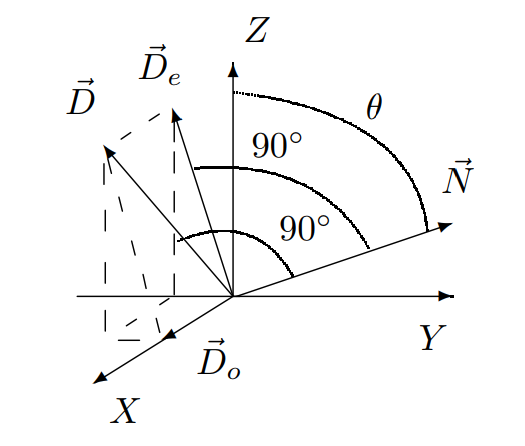
\includegraphics[width = 8cm]{2}}
	\caption{Расположение векторов $\vec{N}$ и $\vec{D}$ в анизотропной среде: $(\vec{D} = \vec{D_o} + \vec{D_e}; \vec{D_o}\perp\vec{D_e}; \vec{D}\perp\vec{N});$
			 $\vec{N}$ и $\vec{D_e}$ лежат в плоскости $(Z,Y)$; $\vec{D_o}$ перпендикулярен плоскости $(Z,Y)$}
	\label{fig:image}
\end{figure}

Волну, распространяющуюся в одноосном кристалле, можно
разделить на две линейно
поляризованные волны: обыкновенную,
вектор электрической индукции
$\vec{D_o}$ которой перпендикулярен
главному сечению, и необыкновенную, с вектором
электрической индукции $\vec{D_e}$, лежащим
в главном сечении (рис. 2).
\textsl{Главным сечением кристалла}
называется плоскость, в которой
лежит оптическая ось кристалла
и нормаль к фронту волны.

Рассмотрим вначале обыкновенную волну, в которой вектор
$\vec{D_o}$ перпендикулярен главному сечению.
Тогда $D_{oz} = 0$, и из условия $D_z = \varepsilon_zE_z$ следует, что $E_{oz} = 0$.

Кроме того, так как $D_{oy} = \varepsilon_\perp E_{oy}$ и $D_{ox} = \varepsilon_\perp E_{ox}$, то можно записать
\begin{equation}
	\vec{D_o} = \varepsilon_\perp\vec{E_o}
\end{equation}

Таким образом, для обыкновенной волны материальное уравнение
имеет такой же вид, как и в изотропной среде. Найдем с помощью этого
уравнения скорость распространения обыкновенной волны
и соответствующий показатель преломления. Из (2) имеем
$$
	D_o = \frac{c}{v_o}H_o,~~H_o = \frac{c}{v_o}E_o
$$
\noindent или, учитывая (5),
$$
	\varepsilon\perp E_o = \frac{c}{v_o}H_o,~~H_o = \frac{c}{v_o}E_o
$$
\noindent откуда
$$
	v_o = \frac{c}{\sqrt{\varepsilon_\perp}},~~n_o = \frac{c}{v_o} = \sqrt{\varepsilon_\perp}
$$

Таким образом, скорость распространения обыкновенной волны
и ее показатель преломления не зависят от направления распространения.

У необыкновенной волны вектор $\vec{D_e}$ не параллелен $\vec{E_e}$, и связь между
ними сложнее, чем в (5).

Для того чтобы найти скорость распространения $v$ и показатель преломления необыкновенной волны
$n = c/v$, достаточно найти связь между вектором электрической индукции этой волны $\vec{D_e}$ и проекцией на него
вектора электрического поля волны $E_{eD}$. Тогда, подставляя
$D_e = \varepsilon E_{eD}$ в (2), приходим
к соотношениям
$$
	\varepsilon E_{eD} = \frac{c}{v}H_e;~~\varepsilon H_e = \frac{c}{v}H_{eD}
$$
\noindent формально тождественным с соотношениями для обыкновенной волны.
Роль величины $\varepsilon_perp$ теперь играет величина $\varepsilon$, а показатель преломления
необыкновенной волны равен $\sqrt{\varepsilon}$.

Найдем связь между $D_e$ и $E_{eD}$. Для этого разложим векторы
$\vec{D_e}$ и $\vec{E_e}$ на составляющие, параллельные и перпендикулярные оси кристалла:
$$
	\vec{D_e} = \vec{D_{||}} + \vec{D_\perp}
$$
$$
	\vec{E_e} = \vec{E_{||}} + \vec{E_\perp}
$$

Учитывая (4), находим
$$
	E_{eD} = \frac{\vec{E_e}\vec{D_e}}{D_e} = \frac{\vec{E_{e||}}\vec{D_{e||}} + \vec{E_{e\perp}}\vec{D_{e\perp}}}{D_e} = 
	\frac{D_{e||}^2/\varepsilon_{||} + D_{e\perp}^2/\varepsilon_\perp}{D_e}
$$
\noindent или
$$
	E_{eD} = D_e\left(\frac{\sin^2\theta}{\varepsilon_{||}} + \frac{\cos^2\theta}{\varepsilon_\perp}\right) = \frac{D_e}{\varepsilon}
$$
\noindent где $\theta$ -- угол между оптической осью $Z$ и волновой нормалью $N$ (рис. 2):
\begin{equation}
	\sin\theta = \frac{D_{e||}}{d_e},~~\cos\theta = \frac{D_{e\perp}}{D_e}
\end{equation}

Таким образом, $\varepsilon$ и, соответственно, скорость распространения и показатель
преломления необыкновенной волны зависят от угла между оптической
осью кристалла и направлением распространения волны.

Выпишем выражение для показателя преломления необыкновенной волны
$n = \sqrt{\varepsilon}$ через главные показатели преломления
$n_o$, $n_e$ и угол $\theta$:
\begin{equation}
	\frac{1}{[n(\theta)]^2} = \frac{\sin^2\theta}{n_e^2} + \frac{\cos^2\theta}{n_o^2}
\end{equation}

При $n_o - n_e \ll n_o $ и $n_e$ (для исландского шпата $n_o = 1.655$, $n_e = 1.485$ для $\lambda = 0.63$ мкм) (7) можно упростить:
\begin{equation}
	n_\theta \approx n_e + (n_o - n_e)\cos^2\theta
\end{equation}

\textbf{Двойное лучепреломление в призме из исландского шпата.}
Рассмотрим, как по преломлению лучей в кристаллической призме можно
определить показатели преломления для обыкновенной и необыкновенной волны.
В работе исследуется одна из двух призм, составляющих поляризатор (рис. 3).

\begin{figure}[h!]
	\center{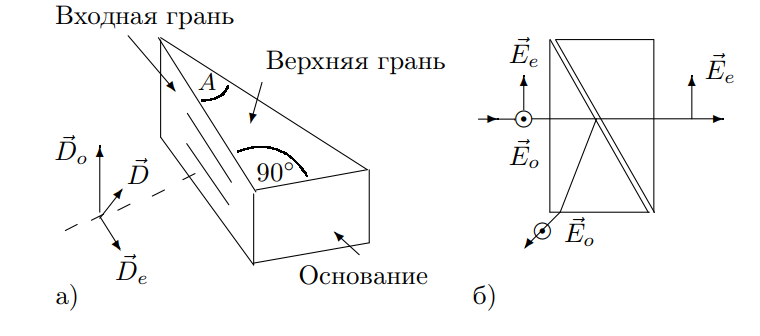
\includegraphics[width = 13cm]{3}}
	\caption{a) исследуемая призма из исландского шпата. Штриховой линией указано направление оптической оси кристалла. б) Ход лучей в поляризационной линзе}
	\label{fig:image}
\end{figure}

В исследуемой призме ось кристалла лежит в плоскости, параллельной
верхней грани призмы, причем она параллельна входной грани призмы (длинному катету). При этом в обыкновенной волне вектор
$\vec{D_o}$ перпендикулярен верхней грани призмы,
а в необыкновенной волне вектор $\vec{D_e}$ параллелен верхней грани.

\begin{figure}[h!]
	\center{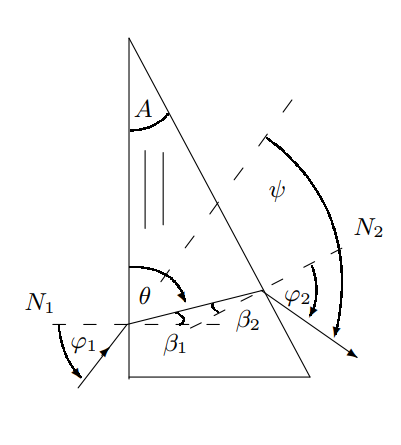
\includegraphics[width = 8cm]{4}}
	\caption{Ход лучей в призме}
	\label{fig:image}
\end{figure}

Волну, падающую на входную грань
призмы, можно представить в виде
суммы двух ортогональных линейно
поляризованных волн. Преломление
этих двух волн на грани призмы можно
рассматривать независимо. Волна,
в которой вектор $\vec{D}$ направлен вертикально
(перпендикулярно верхней грани и оси кристалла), внутри кристалла
будет распространяться как обыкновенная.
Для этой волны выполняется
закон Снеллиуса, а показатель преломления
призмы для нее равен $n_o = \sqrt{\varepsilon_\perp}$. Волна, в которой вектор
$\vec{D}$ направлен горизонтально, в кристалле
будет распространяться
как необыкновенная.
Для этой волны также будет выполняться закон Снеллиуса, но
с тем отличием, что показатель преломления призмы для нее будет зависеть
от угла между осью кристалла и волновой нормалью.

Значение показателя преломления и угол, под которым преломилась
волна в призме, можно найти, измерив угол падения на входную грань
призмы $\varphi_1$ и угол $\varphi_2$ на выходе призмы (рис. 4). Запишем закон Снеллиуса
для одной из волн применительно к первой и второй граням призмы:
$$
	\sin\varphi_1 = n\sin\beta_1
$$
$$
	\sin\varphi_2 = n\sin\beta_2 = n\sin(A - \beta_1).
$$
\noindent При этом мы выразили угол падения на вторую грань призмы $\beta_2$ через
угол преломления на первой грани призмы $\beta_1$ и угол при вершине призмы
$A$. Как видно из рис. 4, эти углы связаны простым соотношением
$A = \beta_1 + \beta_2$. Учитывая, что угол преломления $\beta_1$ связан с углом $\theta$ между осью кристалла
и волновой нормалью $\vec{N}$ соотношением $\theta + \beta_1 = \pi/2$, находим $n$ и $\theta$:
\begin{equation}
	n = \frac{1}{\sin A}\sqrt{\sin^2\varphi_1 + \sin^2\varphi_2 + 2\sin\varphi_1\sin\varphi_2\cos A}
\end{equation}
$$
	\cos\theta = \frac{\sin\varphi_1}{n}
$$
\noindent Для обыкновенной волны
$n$ не будет зависеть от угла $\theta$, а для необыкновенной
волны зависимость $n$ от $\theta$ должна описываться выражением (7).

Показатель преломления призмы из изотропного материала удобно
находить по углу наименьшего отклонения луча от первоначального направления.
Угол отклонения луча призмой ($\psi$ на рис. 4) минимален для симметричного
хода лучей, т.е. когда $\varphi_1 = \varphi_2$. Тогда показатель преломления
можно рассчитать по формуле
\begin{equation}
	n = \frac{\sin\left(\frac{\psi_m + A}{2}\right)}{\sin\left(\frac{A}{2}\right)}
\end{equation}

\noindent где $\psi_m$ -- угол наименьшего отклонения.

Если призма неизотропна, то этой формулой, строго говоря, можно
воспользоваться только для обыкновенной волны,
которая, как это было показано ранее, распространяется так же, как
и в изотропной среде. Но если учесть, что угол при вершине призмы мал,
и при угле наименьшего отклонения преломлённый луч в призме распространяется под углом к
оси кристалла, близким к $\pi/2$, то в качестве оценки формулу (10) можно использовать для определения
$n_e$.


\textbf{Экспериментальная установка.} Схема экспериментальной установки
изображена на рис. 5. Источником излучения служит $Не-Nе$ лазер ($\lambda = 0.63$ мкм). Излучение лазера поляризовано линейно за счет наличия
брюстеровских окошек в кювете лазера. Направление вектора $\vec{E}$ в луче можно изменять с помощью поляроида, установленного на выходе
лазера. Исследуемая призма из исландского шпата закреплена в центре поворотного столика с неподвижным лимбом для отсчета углов.

Преломляющий угол $A$ призмы (рис. 4) можно рассчитать, если известны
угловые координаты нормалей
$N_1$ и $N_2$ к \textsl{преломляющим (рабочим)} граням призмы, прилежащим преломляющему углу. Грань, противолежащая
преломляющему углу, называется \textsl{основанием} призмы. Штриховкой указано направление оптической оси.

Обычно ход лучей в призме таков, что и падающий,
и преломлённый лучи отклоняютс я от нормалей в сторону основания призмы, при этом углы
$\varphi_1$ и $\varphi_2$ считаются положительными.

Угол падения $\varphi_1$ определяется по положению луча, отражённого от передней (входной) грани призмы (рис. 5). Из рис. 4 можно получить
связь углов $\varphi_1$ и $\varphi_2$:
\begin{equation}
	\varphi_2 = A + \psi - \varphi_1
\end{equation}

\noindent а угол $\psi$ -- отклонение преломлённого луча от первоначального направления -- определяется по разности отсчётов на лимбе между точками,
куда попадает луч в отсутствие призмы, и точкой, куда попадает преломлённый
луч.

\begin{figure}[h!]
	\center{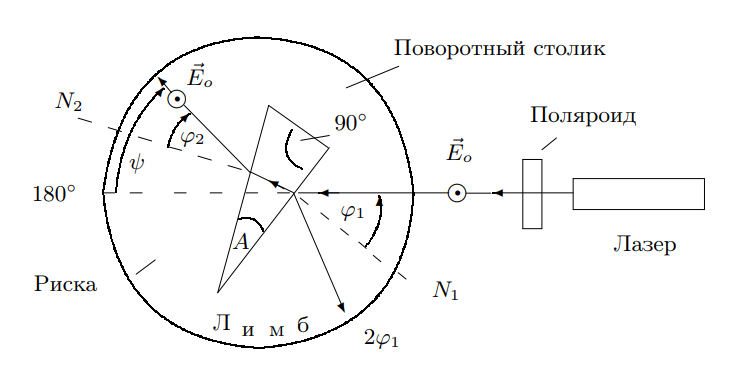
\includegraphics[width = 13cm]{5}}
	\caption{Схема экспериментальной установки}
	\label{fig:image}
\end{figure}

При монотонном увеличении угла падения угол
$\psi$ сначала уменьшается, а затем снова начинает увеличиваться. Минимальное отклонение
соответствует симметричному ходу луча: внутри призмы луч идёт перпендикулярно
биссектрисе угла $A$, а $\varphi_1 = \varphi_2$. Углы наименьшего отклонения
$\psi_m$ различны для обыкновенного и необыкновенного лучей.

Угол $A$ подобран так, что призма может выполнять роль поляризатора:
при нормальном падении луча на первую преломляющую грань
из призмы выходит только один луч, а другой испытывает полное внутреннее
отражение на второй грани. При повороте призмы на небольшой угол на экране появляются оба преломлённых луча. Можно подобрать
такой угол падения, при котором исчезнет второй преломлённый
луч. Область углов поворота призмы, в которой обеспечивается пространственное
разделение лучей с взаимно ортогональной поляризацией, определяется относительной разницей главных показателей преломления
$n_o$ и $n_e$.

\newpage
\textbf{Ход работы.}

1. Отъюстируем и закрепим установку.

2. Определим угол $A$ при вершине призмы. Для этого определим положение засечки при нормальном падении луча на прилегающие к углу стороны:
$$
	\varphi_1 = 289^\circ,~~\varphi_2 = 152^\circ
$$
Откуда
$$
	A = 180^\circ - (\varphi_1 - \varphi_2) = 39^\circ
$$
Оценивая погрешность измерений как $1^\circ$, получим
$$
	A = (39 \pm 2)^\circ
$$

3. Снимем зависимость $180+\psi$ от $2\varphi_1$ для обыкновенной (вертикальная поляризация) и необыкновенной (горизонтальная поляризация) волн:

\begin{center}
\begin{tabular}{|c|c|c|c|c|c|c|c|c|c|c|c|c|c|c|c|}
\hline
\multicolumn{2}{|c|}{обыкновенная}					&	\multicolumn{2}{|c|}{необыкновенная}				\\
\hline
$2\varphi_1, ^\circ$	&	$(180 + \psi), ^\circ$	&	$2\varphi_1, ^\circ$	&	$(180 + \psi), ^\circ$	\\
\hline
20						&	214						&	20						&	202						\\
\hline
25						&	211						&	25						&	202						\\
\hline
30						&	210						&	30						&	201						\\
\hline
35						&	210						&	35						&	201						\\
\hline
40						&	208						&	40						&	201						\\
\hline
45						&	208						&	45						&	200						\\
\hline
50						&	207						&	50						&	200						\\
\hline
55						&	207						&	55						&	200						\\
\hline
60						&	207						&	60						&	200						\\
\hline
65						&	207						&	65						&	200						\\
\hline
70						&	207						&	70						&	201						\\
\hline
75						&	207						&	75						&	201						\\
\hline
80						&	207						&	80						&	201						\\
\hline
85						&	208						&	85						&	202						\\
\hline
90						&	208						&	90						&	203						\\
\hline
95						&	209						&	95						&	203						\\
\hline
100						&	210						&	100						&	204						\\
\hline
105						&	210						&	105						&	205						\\
\hline
110						&	211						&	110						&	205						\\
\hline
115						&	212						&	115						&	206						\\
\hline
120						&	213						&	120						&	207						\\
\hline
125						&	214						&	125						&	209						\\
\hline
130						&	215						&	130						&	210						\\
\hline
135						&	217						&	135						&	212						\\
\hline
140						&	218						&	140						&	213						\\
\hline
\end{tabular}
\end{center}


При этом по-прежнему оценим погрешность прямых измерений как $1^\circ$. Тогда:

\vspace{0.5cm}
Для обыкновенной волны
\begin{center}
\begin{tabular}{|c|c|c|c|c|c|c|c|c|c|c|c|c|c|c|}
\hline
$\phi_1, ^\circ$	&	$\psi, ^\circ$	&	$\phi_1, rad$	&	$\psi, rad$	&	$\phi_2, rad$	&	$n_\text{обыкн}$	&	$cos\theta$	&	$\cos^2\theta$	\\
\hline
10,0&34&0,17&0,59&1,10&1,64&0,11&0,01\\
\hline
12,5&31&0,22&0,54&1,00&1,62&0,13&0,02\\
\hline
15,0&30&0,26&0,52&0,94&1,63&0,16&0,03\\
\hline
17,5&30&0,31&0,52&0,90&1,64&0,18&0,03\\
\hline
20,0&28&0,35&0,49&0,82&1,62&0,21&0,04\\
\hline
22,5&28&0,39&0,49&0,78&1,63&0,23&0,05\\
\hline
25,0&27&0,44&0,47&0,72&1,62&0,26&0,07\\
\hline
27,5&27&0,48&0,47&0,67&1,63&0,28&0,08\\
\hline
30,0&27&0,52&0,47&0,63&1,63&0,31&0,09\\
\hline
32,5&27&0,57&0,47&0,58&1,63&0,33&0,11\\
\hline
35,0&27&0,61&0,47&0,54&1,63&0,35&0,12\\
\hline
37,5&27&0,65&0,47&0,50&1,63&0,37&0,14\\
\hline
40,0&27&0,70&0,47&0,45&1,62&0,40&0,16\\
\hline
42,5&28&0,74&0,49&0,43&1,64&0,41&0,17\\
\hline
45,0&28&0,79&0,49&0,38&1,63&0,43&0,19\\
\hline
47,5&29&0,83&0,51&0,36&1,64&0,45&0,20\\
\hline
50,0&30&0,87&0,52&0,33&1,65&0,46&0,22\\
\hline
52,5&30&0,92&0,52&0,29&1,64&0,48&0,24\\
\hline
55,0&31&0,96&0,54&0,26&1,64&0,50&0,25\\
\hline
57,5&32&1,00&0,56&0,24&1,65&0,51&0,26\\
\hline
60,0&33&1,05&0,58&0,21&1,65&0,53&0,28\\
\hline
62,5&34&1,09&0,59&0,18&1,64&0,54&0,29\\
\hline
65,0&35&1,13&0,61&0,16&1,64&0,55&0,31\\
\hline
67,5&37&1,18&0,65&0,15&1,66&0,56&0,31\\
\hline
70,0&38&1,22&0,66&0,12&1,65&0,57&0,33\\
\hline
\end{tabular}
\end{center}

\newpage
И для необыкновенной:
\begin{center}
\begin{tabular}{|c|c|c|c|c|c|c|c|c|c|c|c|c|c|c|}
\hline
$\phi_1, ^\circ$	&	$\psi, ^\circ$	&	$\phi_1, rad$	&	$\psi, rad$	&	$\phi_2, rad$	&	$n_\text{необыкн}$	&	$cos\theta$	&	$\cos^2\theta$	\\
\hline
10,0&22&0,17&0,38&0,89&1,46&0,12&0,01\\
\hline
12,5&22&0,22&0,38&0,85&1,47&0,15&0,02\\
\hline
15,0&21&0,26&0,37&0,79&1,47&0,18&0,03\\
\hline
17,5&21&0,31&0,37&0,74&1,48&0,20&0,04\\
\hline
20,0&21&0,35&0,37&0,70&1,48&0,23&0,05\\
\hline
22,5&20&0,39&0,35&0,64&1,47&0,26&0,07\\
\hline
25,0&20&0,44&0,35&0,59&1,47&0,29&0,08\\
\hline
27,5&20&0,48&0,35&0,55&1,47&0,31&0,10\\
\hline
30,0&20&0,52&0,35&0,51&1,48&0,34&0,11\\
\hline
32,5&20&0,57&0,35&0,46&1,47&0,36&0,13\\
\hline
35,0&21&0,61&0,37&0,44&1,49&0,38&0,15\\
\hline
37,5&21&0,65&0,37&0,39&1,49&0,41&0,17\\
\hline
40,0&21&0,70&0,37&0,35&1,48&0,43&0,19\\
\hline
42,5&22&0,74&0,38&0,32&1,50&0,45&0,20\\
\hline
45,0&23&0,79&0,40&0,30&1,51&0,47&0,22\\
\hline
47,5&23&0,83&0,40&0,25&1,50&0,49&0,24\\
\hline
50,0&24&0,87&0,42&0,23&1,51&0,51&0,26\\
\hline
52,5&25&0,92&0,44&0,20&1,52&0,52&0,27\\
\hline
55,0&25&0,96&0,44&0,16&1,50&0,55&0,30\\
\hline
57,5&26&1,00&0,45&0,13&1,51&0,56&0,31\\
\hline
60,0&27&1,05&0,47&0,10&1,51&0,57&0,33\\
\hline
62,5&29&1,09&0,51&0,10&1,53&0,58&0,34\\
\hline
65,0&30&1,13&0,52&0,07&1,53&0,59&0,35\\
\hline
67,5&32&1,18&0,56&0,06&1,54&0,60&0,36\\
\hline
70,0&33&1,22&0,58&0,03&1,54&0,61&0,37\\
\hline
\end{tabular}
\end{center}

Погрешность значений $\varphi_1$ равна $0.5^\circ$, погрешность же $\psi$ равна $1^\circ$, откуда, зная, что $\varphi_2 = A + \psi - \varphi_1$, получим, что погрешность $\varphi_2$ равна $3^\circ$. Отсюда погрешность $n$ определим, считая $n = f(A, \varphi_1, \varphi_2)$:
$$
	\sigma_n = \sum\left(\frac{\partial f}{\partial x_i}\sigma_{x_i}\right)^2
$$
Получим:
$$
	\sigma_n = 0.15
$$

Аналогично, найдем погрешность $\cos^2\theta$: $\sigma_\theta = 0.03$.

Построим графики:

\vspace{1cm}
\begin{tikzpicture}
\begin{axis}[
	height = 10cm,
	width  = 15cm,
	every axis y label/.style={at = {(ticklabel cs: 0.5)}, rotate = 90, anchor = near ticklabel},
	xlabel = {$\cos^2\theta$},
	ylabel = {$n$},
	grid   = major
]
\addplot+[
	only marks,
	error bars/.cd, 
	y dir = both, y explicit,
	x dir = both, x explicit,
	]
coordinates{
	(0.01, 1.64)
	(0.02, 1.62)
	(0.03, 1.63)
	(0.03, 1.64)
	(0.04, 1.62)
	(0.05, 1.63)
	(0.07, 1.62)
	(0.08, 1.63)
	(0.09, 1.63)
	
	(0.11, 1.63)
	(0.12, 1.63)
	(0.14, 1.63)
	(0.16, 1.62)
	(0.17, 1.64)
	(0.19, 1.63)
	(0.20, 1.64)
	
	(0.22, 1.65)
	(0.24, 1.64)
	(0.25, 1.64)
	(0.26, 1.65)
	(0.28, 1.64)
	(0.29, 1.64)
	
	(0.31, 1.66)
	(0.31, 1.66)
	(0.33, 1.65)
};


\addplot+[
	only marks,
	error bars/.cd, 
	y dir = both, y explicit,
	x dir = both, x explicit,
	]
coordinates{
	(0.01, 1.46)
	(0.02, 1.47)
	(0.03, 1.47)
	(0.04, 1.48)
	(0.05, 1.48)
	(0.07, 1.47)
	(0.08, 1.47)
	
	(0.10, 1.47)
	(0.11, 1.48)
	(0.13, 1.47)
	(0.15, 1.49)
	(0.17, 1.49)
	(0.19, 1.48)
	
	(0.20, 1.50)
	(0.22, 1.51)
	(0.24, 1.50)
	(0.26, 1.51)
	(0.27, 1.52)
	
	(0.30, 1.50)
	(0.31, 1.51)
	(0.33, 1.51)
	(0.34, 1.53)
	(0.35, 1.53)
	(0.36, 1.54)
	(0.37, 1.54)
};

\addplot [mark = none]
coordinates{
	(0.01, 1.46186)
	(0.37, 1.52928)
};

\addplot [mark = none]
coordinates{
	(0.00, 1.635)
	(0.37, 1.635)
};

\end{axis}
\end{tikzpicture}

Отсюда:
$$
	n_o = 1.63 \pm 0.15
$$
$$
	n_e = 1.48 \pm 0.13
$$

\vspace{1cm}
Найдем также $\psi_m$ для обыкновенной и необыкновенной волн:
$$
	\psi_{m~\text{обыкн}} = 1.63
$$
$$
	\psi_{m~\text{необыкн}} = 1.48
$$

Откуда:
$$
	n_o = 1.63 \pm 0.13
$$
$$
	n_e = 1.48 \pm 0.14
$$


\end{document}
